%%%%%%%%%%%%%%%%%%%%%%%%%%%%%%%%%%%%%%%%%%%%%%%%%%%%%%%%%%%%%%%%%%%%%%%%%%%%%%%%
% DASC 2019 Paper
%%%%%%%%%%%%%%%%%%%%%%%%%%%%%%%%%%%%%%%%%%%%%%%%%%%%%%%%%%%%%%%%%%%%%%%%%%%%%%%%

\documentclass[conference]{IEEEtran}

% The following line is only needed to identify funding in the first footnote.
% If that is unneeded, please comment it out.
\IEEEoverridecommandlockouts

\usepackage{cite}
\usepackage{amsmath,amssymb,amsfonts}
\usepackage{algorithmic}
\usepackage{graphicx}
\usepackage{textcomp}
\usepackage{xcolor}
\usepackage{todonotes}

\def\BibTeX{{\rm B\kern-.05em{\sc i\kern-.025em b}\kern-.08em
  T\kern-.1667em\lower.7ex\hbox{E}\kern-.125emX}}

% Notes, TODOs, etc.
\newcommand{\note}[1]{\textcolor{blue}{#1}}
\renewcommand{\todo}[1]{\textcolor{orange}{#1}}
\newcommand{\done}[1]{\textcolor{green}{#1}}

%%%%%%%%%%%%%%%%%%%%%%%%%%%%%%%%%%%%%%%%%%%%%%%%%%%%%%%%%%%%%%%%%%%%%%%%%%%%%%%%
\begin{document}
%%%%%%%%%%%%%%%%%%%%%%%%%%%%%%%%%%%%%%%%%%%%%%%%%%%%%%%%%%%%%%%%%%%%%%%%%%%%%%%%

\title{
  The Integration of STPA with Domain-Targeted SysML System \& Safety
  Engineering
}

\author{\IEEEauthorblockN{1\textsuperscript{st} Given Name Surname}
\IEEEauthorblockA{\textit{dept. name of organization (of Aff.)} \\
\textit{name of organization (of Aff.)}\\
City, Country \\
email address}
\and
\IEEEauthorblockN{2\textsuperscript{nd} Given Name Surname}
\IEEEauthorblockA{\textit{dept. name of organization (of Aff.)} \\
\textit{name of organization (of Aff.)}\\
City, Country \\
email address}
\and
\IEEEauthorblockN{3\textsuperscript{rd} Given Name Surname}
\IEEEauthorblockA{\textit{dept. name of organization (of Aff.)} \\
\textit{name of organization (of Aff.)}\\
City, Country \\
email address}
\and
\IEEEauthorblockN{4\textsuperscript{th} Given Name Surname}
\IEEEauthorblockA{\textit{dept. name of organization (of Aff.)} \\
\textit{name of organization (of Aff.)}\\
City, Country \\
email address}
\and
\IEEEauthorblockN{5\textsuperscript{th} Given Name Surname}
\IEEEauthorblockA{\textit{dept. name of organization (of Aff.)} \\
\textit{name of organization (of Aff.)}\\
City, Country \\
email address}
\and
\IEEEauthorblockN{6\textsuperscript{th} Given Name Surname}
\IEEEauthorblockA{\textit{dept. name of organization (of Aff.)} \\
\textit{name of organization (of Aff.)}\\
City, Country \\
email address}
}

\maketitle

%-------------------------------------------------------------------------------
\begin{abstract}
%-------------------------------------------------------------------------------
TODO
%-------------------------------------------------------------------------------
\end{abstract}
%-------------------------------------------------------------------------------

%-------------------------------------------------------------------------------
\begin{IEEEkeywords}
%-------------------------------------------------------------------------------
component, formatting, style, styling, insert
%-------------------------------------------------------------------------------
\end{IEEEkeywords}
%-------------------------------------------------------------------------------

%===============================================================================
\section{Introduction}
%===============================================================================

Systems are becoming increasingly connected and interdependent. In parallel
emerging technologies continue to blur the boundary of human and computer
control authority with the level and criticality of computer automation steadily
increasing. To mitigate these risks a broader systems thinking perspective is
needed to support system and safety engineering. Systems Theoretic Process
Analysis (STPA)\cite{leveson2013stpa,leveson2018stpa} is a promising approach to
support and stimulate such thinking. However, today there is little tooling
support that enables the integration of STPA within the broader framework of
system and safety engineering workflows. In this paper, we present an STPA
profile for SCADE Architect. Our goal is that this STPA profile will enable a
cohesive flow down and integration of STPA with domain targeted MBSE SysML
workflows. Through the STPA profile and support environment, we enable the wider
safety context of the target system to be easily modeled. The profile supports
the application of the STPA process, including the capture and association of
STPA fundamentals hazard \& losses, the development and refinement of the
hierarchical control and control loop structures, through assisted Step 1 \&
Step 2, yielding an integrated set of safety requirements and constraints.

The realization of our STPA profile, within the SCADE Architect integrated
workbench, enables all STPA model elements to be allocated and related to
parallel SysML model constructs, which in our case comprise functional, logical
and platform models.

Using the integrated model, it is possible to navigate between the platform
implementation and STPA safety models in both directions. That is to say, within
a few clicks it is possible to rapidly locate the safety context of a detailed
message or logical flow of the system implementation, and vice versa link we can
rapidly traverse to the software and hardware implementation details of the
high-level system control action or feedback flow.

In this paper, we present the design and implementation of the STPA profile
within using the SCADE Architect Configurator. We briefly highlight the
underlying meta models and organization of the profile elements. We also
emphasize to information centric view of the profile construction that is
targeted to ensure information is maintained in a consistent fashion without
duplication. We also explain how our profile has been shaped to align with and
support that natural incremental thinking patterns of typical system safety
engineering.

To illustrate the profile in use, we present a fragment of the STPA analysis of
the wheel brake system from SAE AIR 6110. This work also illustrates the
integration of the STPA, with the principled architectural STPA output. In this
work we also integrate the STPA and traditional safety engineering, leveraging
the SCADE round trip integration bridge with Medini Analyze.

%===============================================================================
\section{Motivation}
%===============================================================================

STPA (System-Theoretic Process Analysis) 
\begin{itemize}
\item New hazard analysis technique 

\item Helps identity by unsafe interactions of system components \& operators

\item Broadens \& compliments traditional component-failure centric approaches

\item Can be used before design is in place 

\end{itemize}
Our view 
\begin{itemize}

\item STPA introduces useful perspectives which can benefit ARP-4754A safety directed system design

\item Helps define architectural drivers  

\item But, we need better process integration \& tooling support 
\end{itemize}

Our vision
\begin{itemize}

\item Integrated STPA, functional and AADL modeling

\item Integrated seamless traceability between system safety context and AADL logical \& physical implementation models 

\end{itemize}

%===============================================================================
\section{SCADE Architect STPA Profile Description}
%===============================================================================

While some tools for STPA already exist (c.f., e.g., \cite{xstampp}), they
suffer from two major problems. First, they are standalone tools, i.e., they
lack the integration within the broader framework of system and safety
engineering workflows. Without this integration, the users are missing one of
the most important features, the traceability between the safety context and the
system implementation. Second, taking into account that STPA is still evolving,
the tools are not flexible enough. In other words, it is hard make any changes
to the way the tools do the STPA if the users need to use even a slightly
different approach. To address both of these problems, we decided to integrate
STPA into the SCADE Architect using the SCADE Configurator tool.

Using the SCADE Configurator, one can create custom UML profiles that can then
be used by SCADE Architect. The profile is generated from a meta-model defined
by the user. This meta-model can reuse and extend constructs from other UML
profiles like, e.g., SysML that is used by SCADE Architect to model the system
architecture. The main advantage of this approach is that it is highly flexible,
i.e., changing how the STPA model should look like means modifying the
meta-model defined in the profile and regenerating the profile, which is quite
easy and quick to do. Figure~\ref{fig:hcs_hierarchy_metamodel} shows a
meta-model defining the hierarchy of elements forming the Hierarchical Control
Structure (HCS) in an STPA model.

\begin{figure}[hbtp]
  \centering
  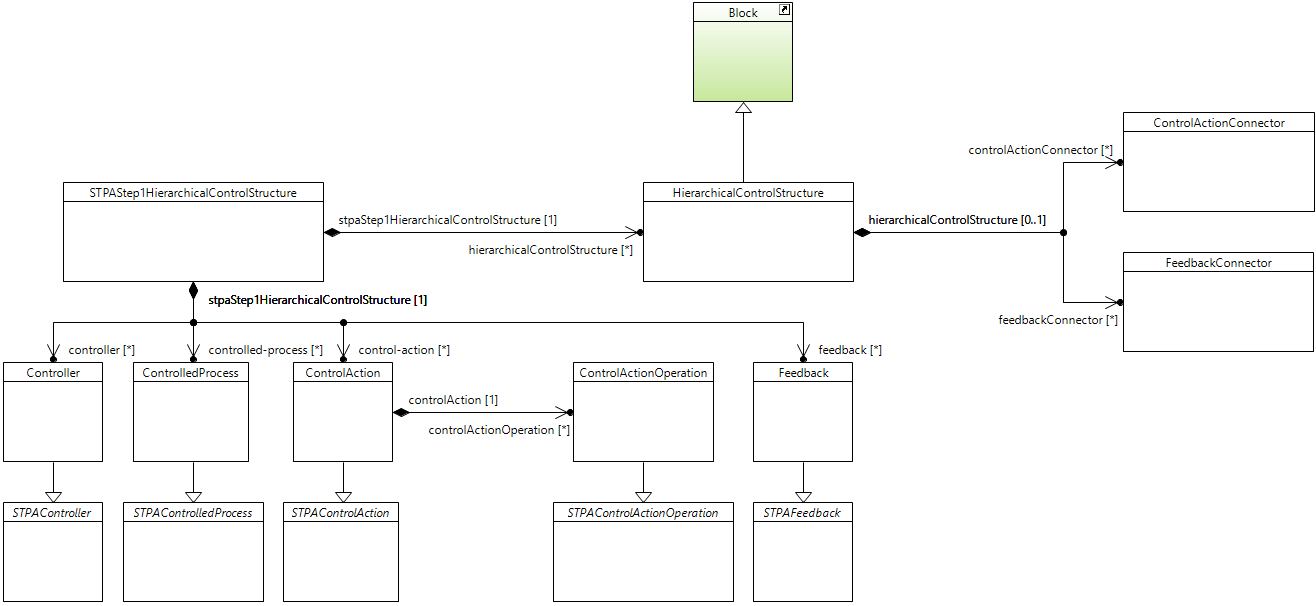
\includegraphics[scale=0.25]{fig/hcs_hierarchy_metamodel.png}
  \caption{STPA profile: meta-model defining HCS hierarchy.}
  \label{fig:hcs_hierarchy_metamodel}
\end{figure}

Using the STPA profile in SCADE Architect then allows us to have both an STPA
model and a model describing the architecture of the system in the same tool.
Moreover, as both models are constructed from SCADE's \texttt{NamedElement}s, we
can link the STPA model elements with SysML model constructs using
\texttt{Allocation}s, establishing a bidirectional traceability between the
system safety and the system implementation.

%-------------------------------------------------------------------------------
\subsection{Hazard and Safety Constraint Refinements}
%-------------------------------------------------------------------------------

For more complex systems, the number of hazards and safety constraints may be
quite large. In such situations, it is often the case that a hazard or a safety
constraint is a more specific version of a generic hazard or safety constraint.
We call such hazards and safety constraints refinements of their generic parents
and our STPA profile allows the user to reflect these parent-child refinement
relationships in the STPA model.

While the refinements are still hazards and safety constraints themselves, and
thus they can have their own requirements, one or two levels of refinements is
usually more then enough even for the most complex systems.

%-------------------------------------------------------------------------------
\subsection{Control Action Operations}
%-------------------------------------------------------------------------------

The Hierarchical Control Structure (HCS) usually contains many control actions,
going from a controller to either another controller or a to controlled process.
While each control action should correctly be represented by a separate control
action connector in the HCS, most of the tools and documents actually associate
all control actions between the same two HCS elements to a single control action
connector. The reason is to prevent clutter in the HCS diagram and as there is
no loss of information (it is known which are the source and target elements of
each control action), it is a safe thing to do.

While we do not have any problem with the mapping of several control actions to
a single control action connector, we see a problem with the modeling of control
actions themselves. The reason is that STPA does not let the user to express
which control actions are independent and which are not. Independent control
actions may occur in parallel in the system.

To address this problem, our STPA profile allows the user to define, for each
control action, a set of its \emph{operations}. An operation can be seen as a
regular control action, however, only a single operation of a control action can
occur at a time. This allows the user to explicitly specify which control
actions are independent (these are represented as standard control actions in
the STPA model) and which are not (these are represented as operations of the
standard control actions).

While it is still possible to map several independent control actions to the
same control action connector in HCS with this approach, it is often not
necessary. There are two reasons for that. The first is that, most of the time,
the control actions are actually not independent, and thus they are modeled as
operations of a specific control action. Then, only a single control action
exists between two HCS elements that needs to be mapped to a control action
connector. The second reason is related to the first one. If independent control
actions are rare, the amount of control action connectors we would remove from
the HCS by mapping several independent control actions to the same control
action connector would be neglible. And, at the same time, we would also remove
a valuable information from the HCS, the information that two control action
connectors are independent and thus may occur in parallel. As a result, our
approach cleans the HCS nicely while keeping all the important information in
it.

%-------------------------------------------------------------------------------
\subsection{Integrating STPA and AADL}
%-------------------------------------------------------------------------------

As we mentioned in the beginning, one of the reasons for integrating STPA into
the SCADE architect is to be able to establish a mapping between the safety
context (STPA elements) and the system implementation (SysML constructs). While
SCADE Architect uses SysML to describe the implementation of a system, it does
not mean it can't utilize other approaches for defining system architecture like
AADL or FACE. In fact, SCADE Architect already comes with the AADL and FACE
profiles. As they are UML profiles utilizing the SysML constructs, there is no
difference for the user if the target system architecture is described in AADL,
FACE, pure SysML or even in their custom UML profile for SCADE Architect. In all
of the cases, the user will be able to link the STPA model elements with the
concrete components in the system architecture.

For example, take the AADL model of a flight control system shown at
Figure~\ref{fig:aadl_model}. This model is taken from one of the SCADE Architect
Avionics (AADL) profile examples. If the user wants to link the SysML components
present in the model with the elements in his STPA model, she just have to
define \texttt{Allocation}s between them. One option is to use an allocation
table and define the mappings there (see
Figure~\ref{fig:stpa_aadl_allocation_table}). Another option is to define the
allocations in the diagrams visualizing the models. As can be seen in
Figure~\ref{fig:control_loop_with_allocations}, the mappings are shown as
\emph{smart comments} in the diagrams. The smart comments are automatically
generated by the SCADE Architect.

\begin{figure}[hbtp]
  \centering
  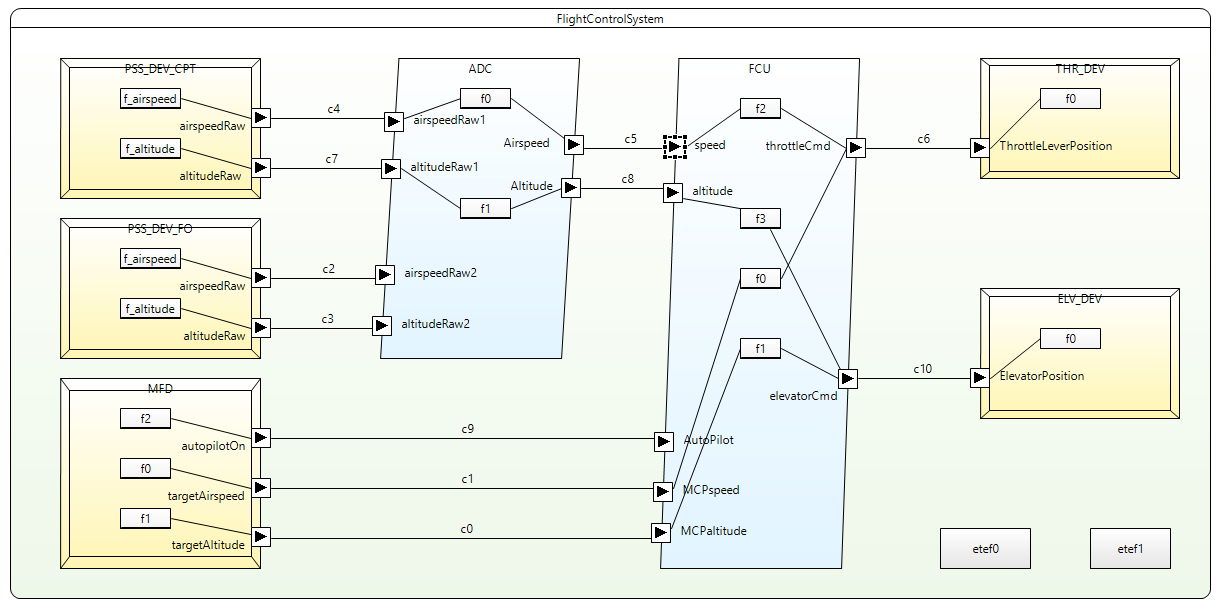
\includegraphics[scale=0.27]{fig/aadl_model.png}
  \caption{AADL model of a flight control system.}
  \label{fig:aadl_model}
\end{figure}

\begin{figure}[hbtp]
  \centering
  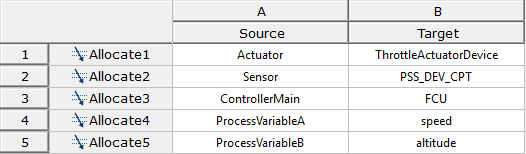
\includegraphics[scale=0.6]{fig/stpa_aadl_allocation_table.png}
  \caption{A table linking STPA elements and SysML construct.}
  \label{fig:stpa_aadl_allocation_table}
\end{figure}

\begin{figure}[hbtp]
  \centering
  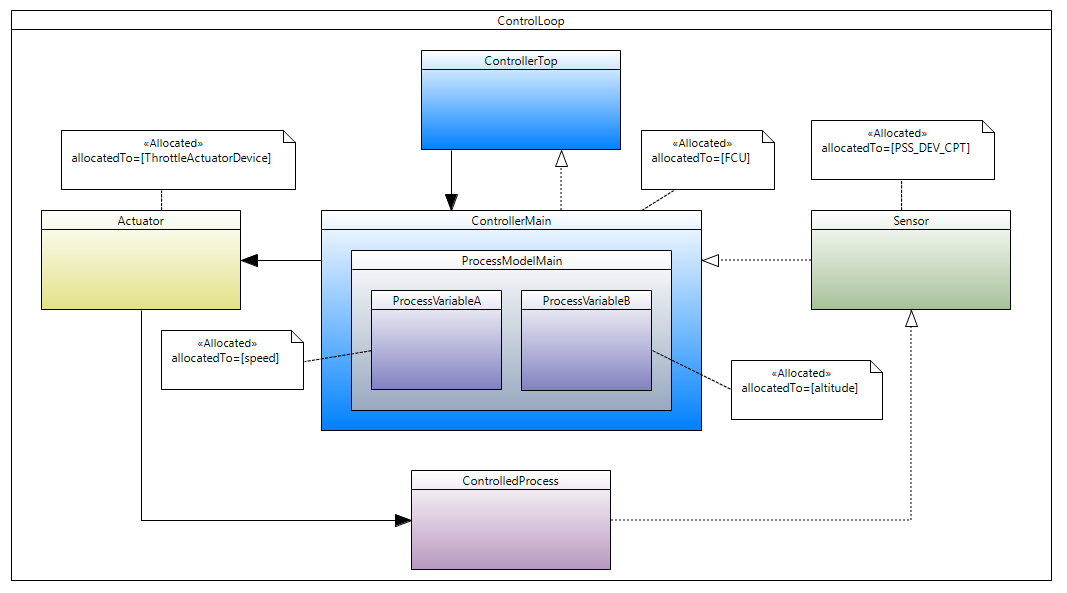
\includegraphics[scale=0.3]{fig/control_loop_with_allocations.png}
  \caption{A control loop with STPA elements mapped to AADL constructs.}
  \label{fig:control_loop_with_allocations}
\end{figure}

Points to consider

\begin{itemize}
\item \done{Flexibility of the configuration}
\item \done{Information-centric approach -- where information flows are
exclusive one arrow}
\item \todo{typing for operations: not sure what that means, data types for
control action operations?}

\item \done{show linkages to architectural model AADL}
\end{itemize}
%===============================================================================
\section{Example of Use}\label{AA}
%===============================================================================

Define abbreviations and acronyms the first time they are used in the text, 
even after they have been defined in the abstract. Abbreviations such as 
IEEE, SI, MKS, CGS, ac, dc, and rms do not have to be defined. Do not use 
abbreviations in the title or heads unless they are unavoidable.

%===============================================================================
\section{Lessons Learned and Discussion}
%===============================================================================
Functional clean view and discipline

\begin{itemize}
\item Flexibility of the configuration
\item STPA Born from CAST where architecture was fixed
\item Looking forward a cleaner functional view may be beneficial - sensing rather than sensor
\item summarize principled architectural refinement 

\end{itemize}



%===============================================================================
\section{Adjacent Work }
%===============================================================================


\begin{itemize}
\item Summarize Medini Profile 

\item  Also mention adjacent  work with model integrated requirements and EARS
\item model decomposition is context for requirements specification
\item Discuss integrated cross cutting requirements context 
\item WHILE operating with anticipated failures, the function shall ....
\item Discuss the basic of cross cutting test generation from integrated model set  

\end{itemize}


%===============================================================================
\section{Future Work}
%===============================================================================

\begin{itemize}
\item Integrate system and safety model is needed 
\item introduce MIDAS
\item move to information model and less focus on point of entry 
\end{itemize}
%-------------------------------------------------------------------------------
\subsection{\LaTeX-Specific Advice}
%-------------------------------------------------------------------------------

%===============================================================================
\section*{Acknowledgment}
%===============================================================================

The preferred spelling of the word ``acknowledgment'' in America is without 
an ``e'' after the ``g''. Avoid the stilted expression ``one of us (R. B. 
G.) thanks $\ldots$''. Instead, try ``R. B. G. thanks$\ldots$''. Put sponsor 
acknowledgments in the unnumbered footnote on the first page.

\bibliographystyle{IEEEtran}
\bibliography{IEEEabrv,stpa}

\vspace{12pt}
\color{red}

IEEE conference templates contain guidance text for composing and formatting
conference papers. Please ensure that all template text is removed from your
conference paper prior to submission to the conference. Failure to remove the
template text from your paper may result in your paper not being published.

%%%%%%%%%%%%%%%%%%%%%%%%%%%%%%%%%%%%%%%%%%%%%%%%%%%%%%%%%%%%%%%%%%%%%%%%%%%%%%%%
\end{document}
%%%%%%%%%%%%%%%%%%%%%%%%%%%%%%%%%%%%%%%%%%%%%%%%%%%%%%%%%%%%%%%%%%%%%%%%%%%%%%%%
